\section{Homogeneous coordinates}

To depict objects in a 3D space effectively, we must select a suitable coordinate system. Homogeneous coordinates are employed for this purpose.

In homogeneous coordinates, a point within the 3D space is defined by four values: $x$, $y$, $z$, and $w$. 
The $x$, $y$, and $z$ coordinates denote the point's position in the 3D space, while the $w$ coordinate determines a scale, influencing the units of measurement utilized by the other three coordinates.
In this system, all coordinates representing the same point (with varying $w$ values) are linearly dependent.

The $x$, $y$, and $z$ coordinates of the vector with $w = 1$ specify the actual position of the point in the 3D space. 
Given that all vectors representing the same point are linearly dependent, we can obtain the one with $w = 1$ by dividing the first three components $(x, y, z)$ by the fourth component, $w$.

We can determine the Cartesian coordinates $(x^\prime,y^\prime,z^\prime)$ corresponding to any point in homogeneous coordinates $(x,y,z,w)$ as follows:
\[(x^\prime,y^\prime,z^\prime)=\left( \dfrac{x}{w},\dfrac{y}{w},\dfrac{z}{w} \right)\]
Conversely, we can straightforwardly convert a point with Cartesian coordinates $(x,y,z)$ into homogeneous coordinates by appending a fourth component $w=1$:
\[(x^\prime,y^\prime,z^\prime)=(x,y,z,1)\]

\begin{figure}[H]
    \centering
    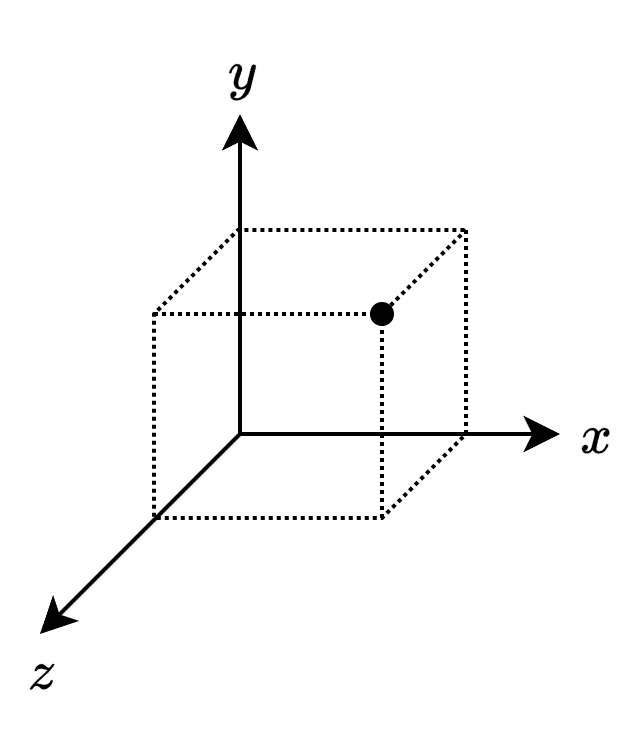
\includegraphics[width=0.23\linewidth]{images/homogeneous.png}
    \caption{Coordinates}
\end{figure}